\subsection{Análisis SHAP}

Después de realizar la investigación y la comparación de algoritmos, se determinó que el mejor modelo de clasificación es RandomForestClassifier, y el mejor modelo de regresión es LinearRegression. A continuación, analizaremos los resultados de estos modelos.

\subsubsection{Análisis del Mejor Modelo de Clasificación: RandomForestClassifier}


Para el análisis, se prepararon las coordenadas de análisis X/Y utilizando la columna \say{aprobado} (binaria, obtenida de \say{sol1}, donde 1 significa aprobado con una nota mayor o igual a 4) como referencia para el eje Y. Analizaremos el comportamiento de las demás columnas en relación con dicho eje X.

\begin{figure}[H]
    \centering
    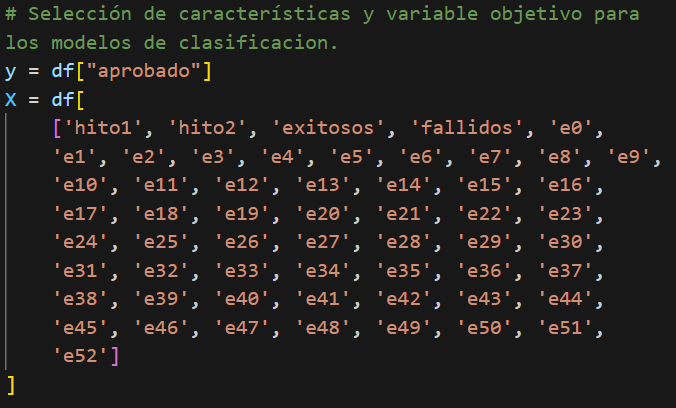
\includegraphics[width=0.5\textwidth]{img/shap_rf/conjunto_clasificacion.png}
    \caption{Selección de característica y variable objetivo}
    \label{fig:variables_entrenamiento}
\end{figure}

Para comprender mejor los gráficos que veremos a continuación, es necesario entender lo siguiente:

\begin{itemize}
    \item El término \say{higher} se refiere a las instancias que tienen valores más altos en comparación con otras instancias, y tienen un mayor impacto en la probabilidad de ser \say{aprobado}.
    \item El término \say{lower} se refiere a las instancias con valores más bajos de la característica, que tienen un menor impacto en la probabilidad de ser \say{aprobado}.
\end{itemize}

En la Figura \ref{fig:caract_var_shap} se muestra el gráfico de características variables SHAP gráfico.

\begin{figure}[H]
    \centering
    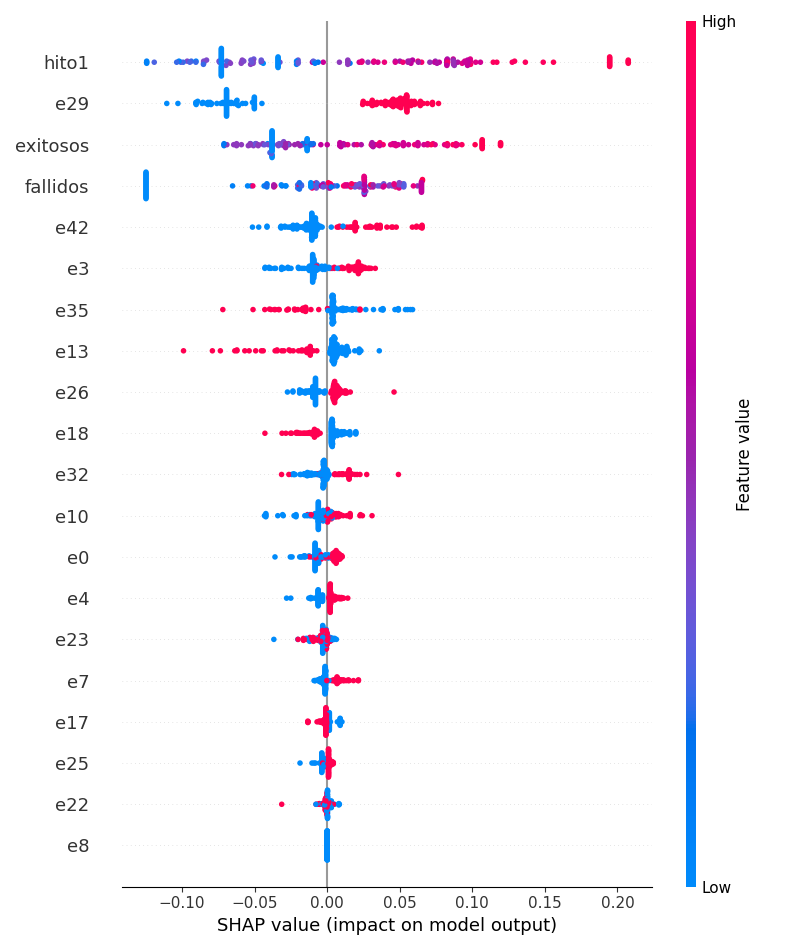
\includegraphics[width=0.5\textwidth]{img/shap_rf/shapForcePlot2.png}
    \caption{Características Variables SHAP}
    \label{fig:caract_var_shap}
\end{figure}

Al observar este podemos destacar lo siguiente:

\begin{itemize}
    \item La variable \say{hito1}  muestra un alto \say{higher} contribuyendo bastante informacion con sus picos de dispercion.
    \item La pregunta de la guía \say{e29} también es una variable de interés, siendo una de las preguntas de la guía con la mayor dispercion en sesgos \say{higher} y \say{lower}.
    \item Tanto las variables \say{exitosos} como \say{fallidos} también son variables interesantes de analizar, ya que están correlacionadas con la intención de resolver la guía.
    \item La variable \say{e42} como la variable \say{e3}, tiene un un conjunto de datos bastante marcado entre  sus colores \say{azul} y \say{rojo}.
\end{itemize}

Además, se presenta otro gráfico generado por matplotlib sobre la prediccion del modelo en la Figura \ref{fig:caract_var_shap_mat}:

\begin{figure}[H]
    \centering
    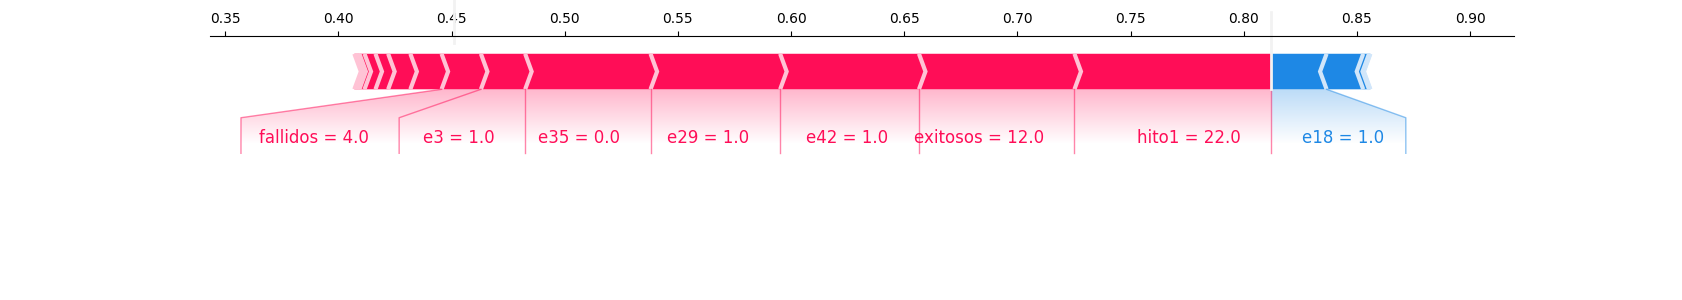
\includegraphics[width=1\textwidth]{img/shap_rf/shapForcePlot.png}
    \caption{Características Variables SHAP (Matplotlib)}
    \label{fig:caract_var_shap_mat}
\end{figure}

Al revisar este gráfico, podemos obtener más detalles sobre las características y su importancia:

\begin{itemize}
    \item La sección \say{higher} muestra los valores positivos que contribuyen a aumentar el valor de predicción. En este caso, \say{hito1} esta mas sercana a la \say{f(x)}, lo que significa que esta característica contribuye positivamente al valor de predicción en conjuntos con las variables \say{exitosos}, \say{e42}, \say{e29}, \say{e35}, \say{e3}, \say{fallidos} para \say{aprobado}.
    \item La sección \say{lower} muestra los valores negativos o fallidos que contribuyen a disminuir el valor de predicción. En este caso, la variable \say{e18}, tiene una contribución negativa al valor de prediccióno que no aporta mucho.
    \item En el gráfico, la marca \say{f(x)} representa el valor de predicción del modelo, que en este caso es 0.81.
\end{itemize}

Además de los gráficos anteriores, se presentan los gráficos de dependencia para algunas variables con referencia a \say{aprobado}:

\begin{figure}[H]

    \begin{subfigure}{0.5\textwidth}
        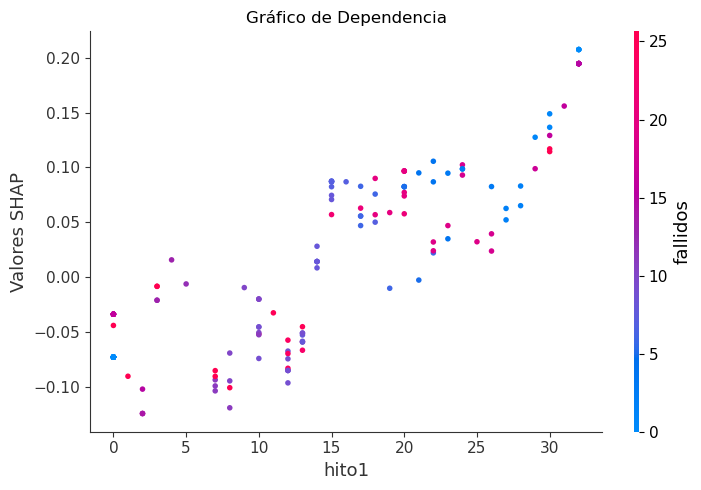
\includegraphics[width=0.9\linewidth, height=6cm]{img/shap_rf/hito1.png}
        \caption{hito1}
        \label{fig:dependencia_hito1}
    \end{subfigure}
    \begin{subfigure}{0.5\textwidth}
        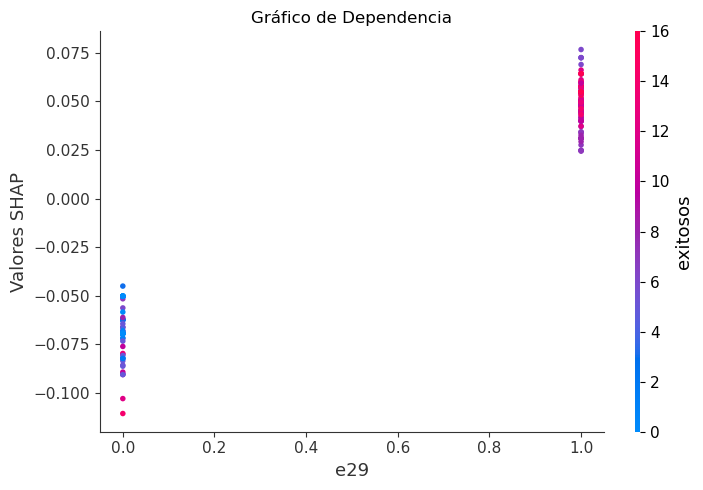
\includegraphics[width=0.9\linewidth, height=6cm]{img/shap_rf/e29.png}
        \caption{e29}
        \label{fig:dependencia_e29}
    \end{subfigure}

    \caption{Variables de dependencias hito1 - e29}
    \label{fig:image2}
\end{figure}

En la Figura \ref{fig:dependencia_hito1} se muestra el gráfico de dependencia para la variable \say{hito1} y refleja \say{fallidos} con su correlación. mientras tanto en la figura \ref{fig:dependencia_e29} se muestra el gráfico de dependencia para la variable \say{e29} con la variable \say{extisoso}.

\begin{figure}[H]

    \begin{subfigure}{0.5\textwidth}
        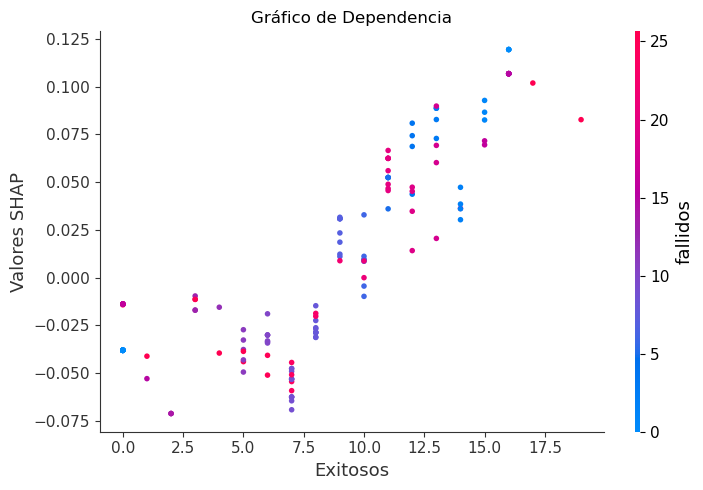
\includegraphics[width=0.9\linewidth, height=6cm]{img/shap_rf/exitosos.png}
        \caption{exitosos}
        \label{fig:dependencia_exitosos}
    \end{subfigure}
    \begin{subfigure}{0.5\textwidth}
        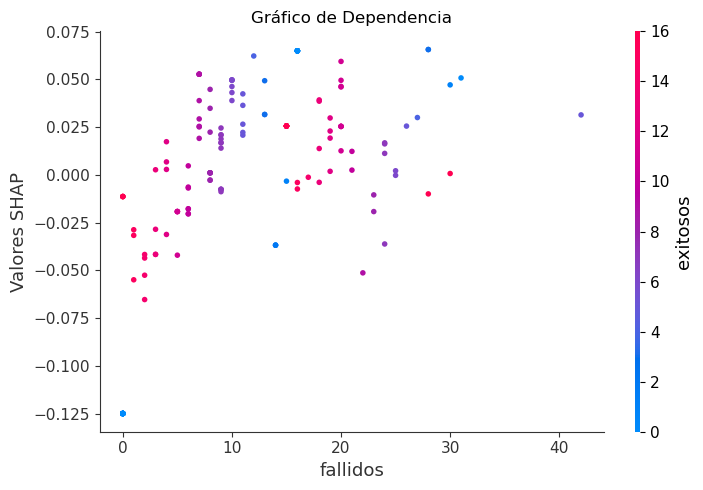
\includegraphics[width=0.9\linewidth, height=6cm]{img/shap_rf/fallidos.png}
        \caption{fallidos}
        \label{fig:dependencia_fallidos}
    \end{subfigure}

    \caption{Variable de dependencias exitosos - fallidos}
    \label{fig:image2}
\end{figure}

En la Figura \ref{fig:dependencia_exitosos} se muestra el gráfico de dependencia para la variable \say{exitosos} con su variable de dependencia \say{fallidos}, mientras tanto en la figura \ref{fig:dependencia_fallidos} se muestra el gráfico de dependencia para la variable \say{fallidos} con su dependencia \say{exitosos}.

\begin{figure}[H]

    \begin{subfigure}{0.5\textwidth}
        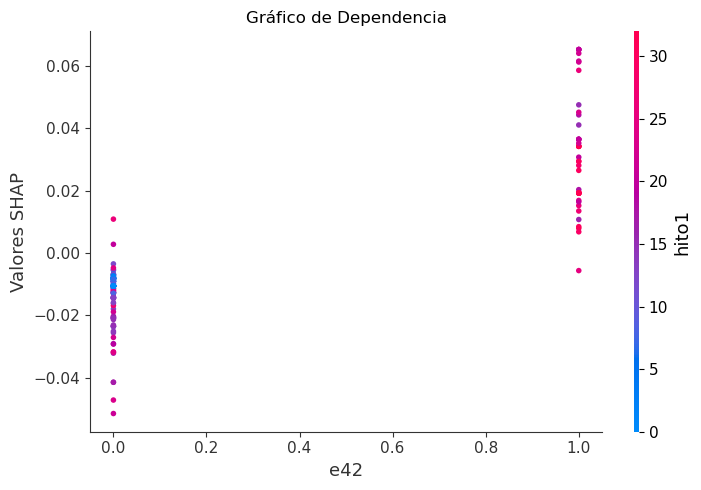
\includegraphics[width=0.9\linewidth, height=6cm]{img/shap_rf/e42.png}
        \caption{e42}
        \label{fig:dependencia_e42}
    \end{subfigure}
    \begin{subfigure}{0.5\textwidth}
        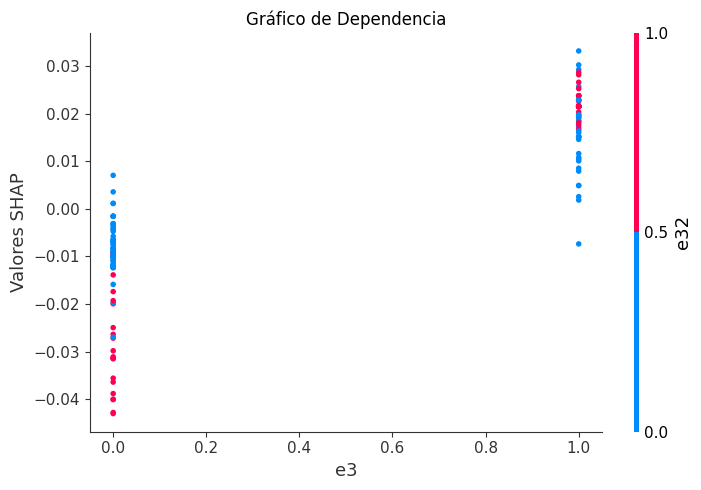
\includegraphics[width=0.9\linewidth, height=6cm]{img/shap_rf/e3.png}
        \caption{e3}
        \label{fig:dependencia_e3}
    \end{subfigure}

    \caption{Variable de dependencias e42 - e3}
    \label{fig:image2}
\end{figure}

En la Figura \ref{fig:dependencia_e42} se muestra el gráfico de dependencia para la variable \say{e42} con su dependencia \say{hito1}, mientras tanto en la figura \ref{fig:dependencia_e3} se muestra el gráfico de dependencia para la variable \say{e3} con la variable \say{e32}.

Estos gráficos de dependencia representan la relación entre los valores de las variables mencionadas y los valores de Shapley en el modelo. Proporcionan una visualización de cómo estas variables influyen en las predicciones del modelo y ayudan a comprender su importancia relativa.

En resumen, podemos entender que el modelo predictivo RandomForestClassifier tiene una función f(x) con una precisión del 81\%. Además, al observar las variables con mayor impacto en la probabilidad de ser clasificado como \textit{aprobado} (denominadas \textit{higher}), encontramos: \textit{hito1}, \textit{exitosos}, \textit{e42}, \textit{e29}, \textit{e35}, \textit{e3} y \textit{fallidos}. Por otro lado, las variables con menor impacto en la probabilidad de ser clasificado como \textit{aprobado} se encuentran en el conjunto \textit{lower}, destacando la variable \textit{e18}.

% \subsubsection{Análisis del Mejor Modelo de Clasificación: LinearRegression}

% Para el análisis, se prepararon las coordenadas de análisis X/Y utilizando la columna \say{sol1} cual representa la nota obtenida en la primera evaluacion, esta parte de la nota 0.0 hasta la nota mas alta 7.0 y para probar se requiere una nota igual o superior a 4.0 como referencia para el eje Y. Analizaremos el comportamiento de las demás columnas en relación con dicho eje X.

% \begin{figure}[H]
%     \centering
%     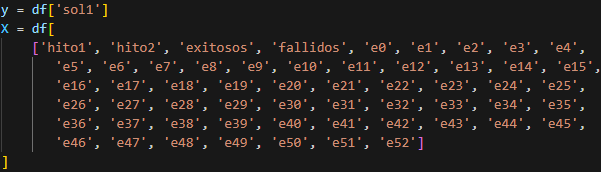
\includegraphics[width=0.5\textwidth]{img/shap_lr/dependencia_variable_objetivo.png}
%     \caption{Selección de característica y variable objetivo}
%     \label{fig:variables_entrenamiento_lr}
% \end{figure}

% En la Figura \ref{fig:caract_var_shap_lr1} se muestra el gráfico de características variables SHAP:

% \begin{figure}[H]
%     \centering
%     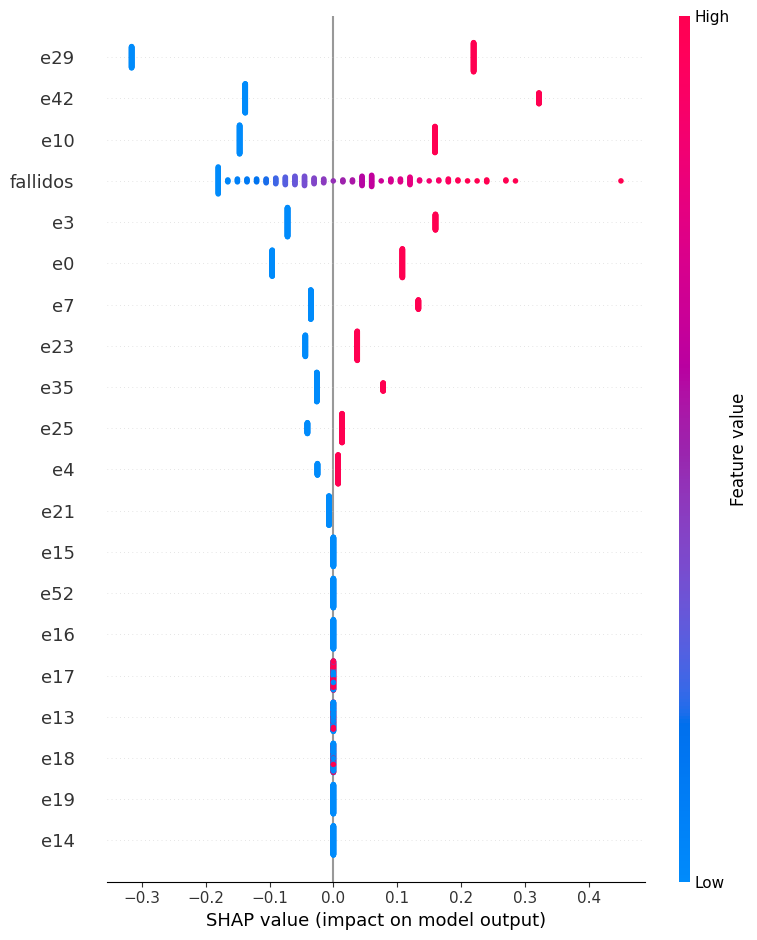
\includegraphics[width=0.5\textwidth]{img/shap_lr/shapForcePlot_lr.png}
%     \caption{Características Variables SHAP}
%     \label{fig:caract_var_shap_lr1}
% \end{figure}

% Al observar este gráfico, podemos destacar lo siguiente:

% \begin{itemize}
%     \item La pregunta de la guía \say{e29} tiene característica con una gama de valores en el conjunto de datos que contribuye significativamente a las predicciones del modelo.
%     \item Como tambien la pregunta de la guía \say{e42} tiene característica que influencian de manera importante en las predicciones y que hay una muestra particular que se ve afectada de manera notable.
%     \item Mientras tanto la pregunta de la guia \say{e10} muestra un sesgo azul y rojo mas sercanos. Esto indica que esta característica tiene una contribución más uniforme en las predicciones y que hay menos variabilidad en los valores de esta característica en el conjunto de datos.
%     \item \say{fallidos} muestra sesgos o puntos que van desde azul hasta rojo. Esto indica que esta característica tiene una amplia gama de valores en el conjunto de datos y contribuye significativamente a las predicciones del modelo.
% \end{itemize}

% Además, se presenta otro gráfico generado por matplotlib en la Figura \ref{fig:caract_var_shap_mat_lr2}:

% \begin{figure}[H]
%     \centering
%     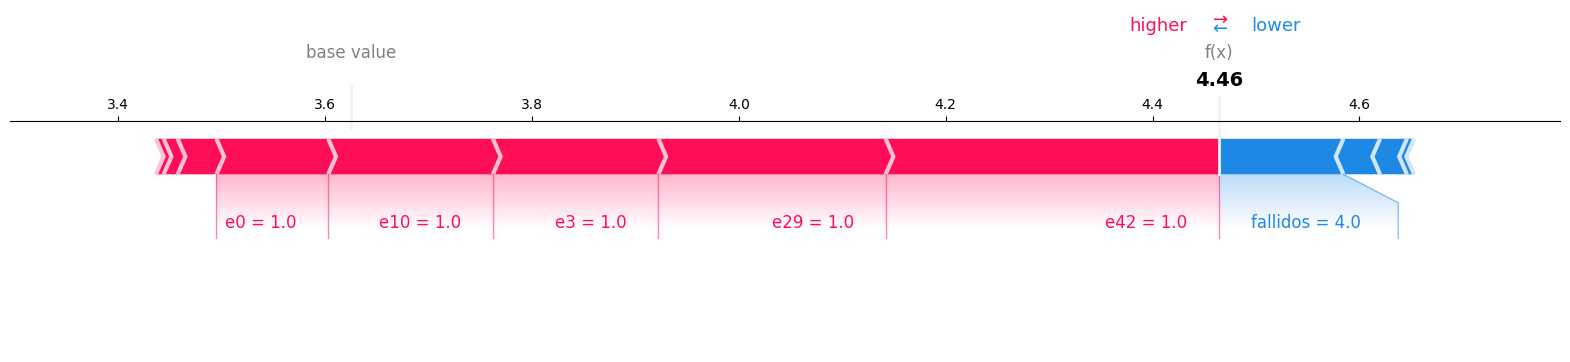
\includegraphics[width=1\textwidth]{img/shap_lr/shapForcePlot_lr2.png}
%     \caption{Características Variables SHAP (Matplotlib)}
%     \label{fig:caract_var_shap_mat_lr2}
% \end{figure}

% Al revisar este gráfico, podemos obtener más detalles sobre las características y su importancia:

% \begin{itemize}
%     \item La sección \say{higher} muestra los \say{e42} o valores positivos que contribuyen a aumentar el valor de predicción. En este caso, la pregunta \say{e42} esta mas sercana a la \say{f(x)}, lo que significa que esta característica contribuye positivamente al valor de predicción en conjuntos con las variables \say{e29}, \say{e3}.
%     \item La sección \say{lower} muestra los valores negativos o fallidos que contribuyen a disminuir el valor de predicción. En este caso, el valor de \say{fallidos} es 4.0, lo que significa que esta característica tiene una contribución negativa al valor de predicción.
%     \item La marca \say{f(x)} en el gráfico representa el valor de predicción del modelo. En este caso, el valor es 4.46\%.
% \end{itemize}



% Además de los gráficos anteriores, se presentan los gráficos de dependencia para algunas variables:

% \begin{figure}[H]

%     \begin{subfigure}{0.5\textwidth}
%         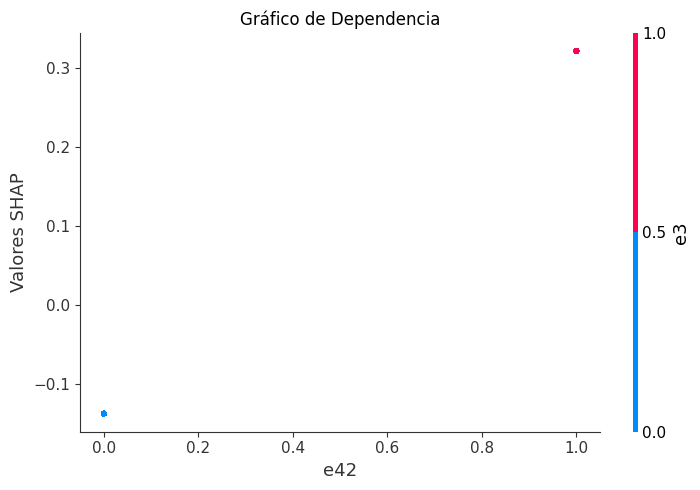
\includegraphics[width=0.9\linewidth, height=6cm]{img/shap_lr/e42.png}
%         \caption{e42}
%         \label{fig:dependencia_e42_lr}
%     \end{subfigure}
%     \begin{subfigure}{0.5\textwidth}
%         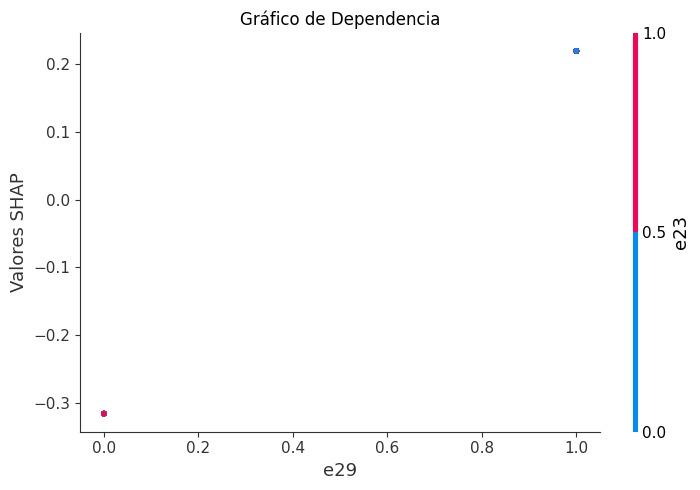
\includegraphics[width=0.9\linewidth, height=6cm]{img/shap_lr/e29.png}
%         \caption{e29}
%         \label{fig:dependencia_e29_lr}
%     \end{subfigure}

%     \caption{Variables de dependencias e42 - e29}
%     \label{fig:image2}
% \end{figure}

% En la Figura \ref{fig:dependencia_e42_lr} se muestra el gráfico de dependencia para la variable \say{e42}. mientras tanto en la figura \ref{fig:dependencia_e29_lr} se muestra el gráfico de dependencia para la variable \say{e29}

% \begin{figure}[H]

%     \begin{subfigure}{0.5\textwidth}
%         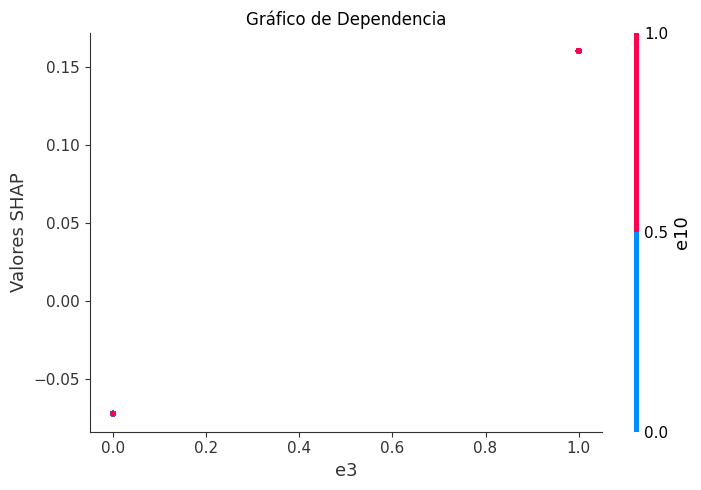
\includegraphics[width=0.9\linewidth, height=6cm]{img/shap_lr/e3.png}
%         \caption{e3}
%         \label{fig:dependencia_e3_lr}
%     \end{subfigure}
%     \begin{subfigure}{0.5\textwidth}
%         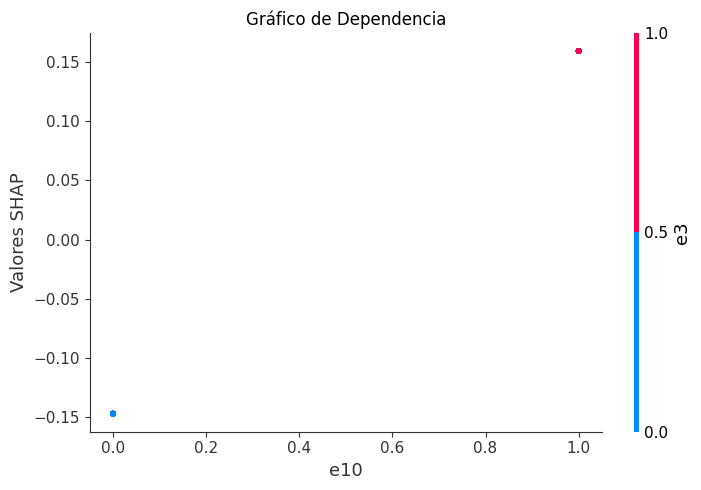
\includegraphics[width=0.9\linewidth, height=6cm]{img/shap_lr/e10.png}
%         \caption{e10}
%         \label{fig:dependencia_e10_lr}
%     \end{subfigure}

%     \caption{Variable de dependencias e3 - e10}
%     \label{fig:image2}
% \end{figure}

% En la Figura \ref{fig:dependencia_e3_lr} se muestra el gráfico de dependencia para la variable \say{e3}, mientras tanto en la figura \ref{fig:dependencia_e10_lr} se muestra el gráfico de dependencia para la variable \say{e10}

% \begin{figure}[H]

%     \begin{subfigure}{0.5\textwidth}
%         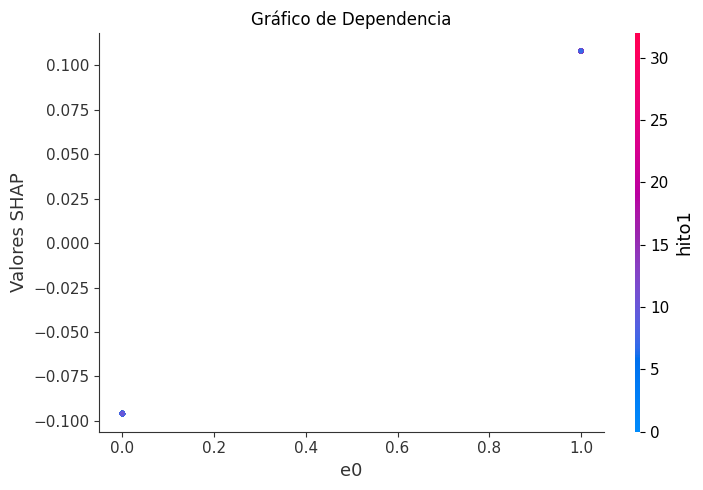
\includegraphics[width=0.9\linewidth, height=6cm]{img/shap_lr/e0.png}
%         \caption{e0}
%         \label{fig:dependencia_e0_lr}
%     \end{subfigure}
%     \begin{subfigure}{0.5\textwidth}
%         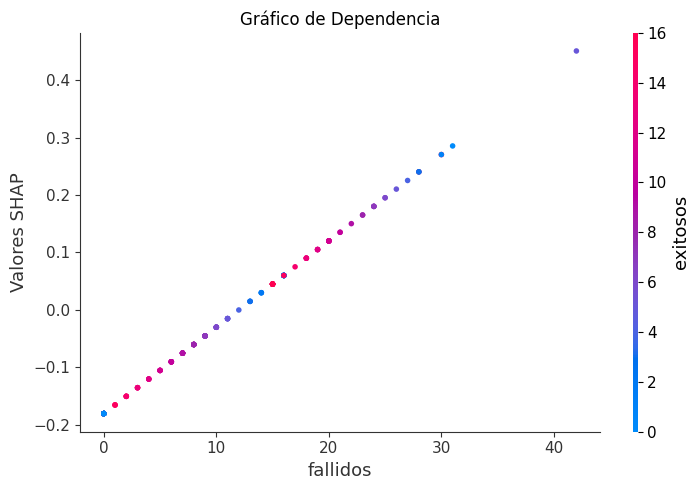
\includegraphics[width=0.9\linewidth, height=6cm]{img/shap_lr/fallidos.png}
%         \caption{fallidos}
%         \label{fig:dependencia_fallidos_lr}
%     \end{subfigure}

%     \caption{Variable de dependencias e0 - fallidos}
%     \label{fig:image2}
% \end{figure}

% En la Figura \ref{fig:dependencia_e0_lr} se muestra el gráfico de dependencia para la variable \say{e0}, mientras tanto en la figura \ref{fig:dependencia_fallidos_lr} se muestra el gráfico de dependencia para la variable \say{fallidos}

% Estos gráficos de dependencia representan la relación entre los valores de las variables mencionadas y los valores de Shapley en el modelo. Proporcionan una visualización de cómo estas variables influyen en las predicciones del modelo y ayudan a comprender su importancia relativa.

En resumen, el análisis SHAP nos ha permitido identificar las características y variables que más influyen en los modelos de clasificación. Esto nos brinda una mejor comprensión de los factores que determinan la resolucion de la guia y la nota obtenida en la prueba de conocimientos.



